\documentclass[conference]{IEEEtran}
\usepackage{amsmath,amssymb}
\usepackage{graphicx}
\usepackage{url}
\usepackage[hidelinks]{hyperref}
\usepackage{booktabs}
\usepackage{array}
\usepackage{dblfloatfix}
\usepackage{adjustbox}
\usepackage{pgfplots}
\usepackage{xcolor}
\definecolor{methodblue}{HTML}{0072B2}
\definecolor{methodorange}{HTML}{E69F00}
\definecolor{methodgreen}{HTML}{009E73}
\definecolor{methodvermillion}{HTML}{D55E00}
\definecolor{methodpurple}{HTML}{CC79A7}
\pgfplotsset{compat=1.18}
\usepgfplotslibrary{groupplots}
\providecommand{\tightlist}{}
\title{Transportability of Post-Hoc Reliability Signals for Network Intrusion Detection under Source-Only Cross-Domain Transfer}
\author{
\IEEEauthorblockN{Shreyas Gautam}
\IEEEauthorblockA{\textit{Department of CSE (AI \& ML)} \\
\textit{Apex Institute of Technology} \\
\textit{Chandigarh University} \\
Gharuan, Mohali -- 140413, India \\
gautamshreyas4@gmail.com}
\and
\IEEEauthorblockN{Bhawika Panchal}
\IEEEauthorblockA{\textit{Department of CSE (AI \& ML)} \\
\textit{Apex Institute of Technology} \\
\textit{Chandigarh University} \\
Gharuan, Mohali -- 140413, India \\
bhawika343@gmail.com}
\and
\IEEEauthorblockN{Himanshi Mittal}
\IEEEauthorblockA{\textit{Department of CSE (AI \& ML)} \\
\textit{Apex Institute of Technology} \\
\textit{Chandigarh University} \\
Gharuan, Mohali -- 140413, India \\
himanshimittalnano2005@gmail.com}
\and
\IEEEauthorblockN{Anna Taneja}
\IEEEauthorblockA{\textit{Department of CSE (AI \& ML)} \\
\textit{Apex Institute of Technology} \\
\textit{Chandigarh University} \\
Gharuan, Mohali -- 140413, India \\
annataneja91@gmail.com}
\and
\IEEEauthorblockN{Aditya Mehta}
\IEEEauthorblockA{\textit{Department of CSE (AI \& ML)} \\
\textit{Apex Institute of Technology} \\
\textit{Chandigarh University} \\
Gharuan, Mohali -- 140413, India \\
adi.mehta002@gmail.com}
\and
\IEEEauthorblockN{Bhupaesh Ghai}
\IEEEauthorblockA{\textit{Department of CSE (AI \& ML)} \\
\textit{Apex Institute of Technology} \\
\textit{Chandigarh University} \\
Gharuan, Mohali -- 140413, India \\
bhupaesh.e16568@cumail.in}
}
\begin{document}
\maketitle
\begin{abstract}
Reliability signals can identify uncertain or potentially erroneous predictions from network intrusion detection systems, but their usefulness may change when a fixed detector is deployed in a different network domain. This study evaluates five source-derived post-hoc reliability signals---calibrated confidence, Random Forest tree disagreement, feature-space distance, split conformal set-size scoring, and Isolation Forest---under strict source-only cross-domain transfer. A fixed Random Forest detector is trained on either NF-UNSW-NB15-v3 or NF-CSE-CIC-IDS2018-v3 using a common 46-feature NetFlow-v3 representation, and the detector and reliability layers are frozen before target scoring. Ten matched seeds are evaluated in both transfer directions. The primary security endpoint is attack-miss AUPRC; operational utility is measured by attack-miss capture at 1\%, 5\%, and 10\% whole-target review budgets.

The in-domain source-test detector is near-perfect, but cross-domain transfer produces severe detector failure: target attack discrimination is close to chance in UNSW$\rightarrow$CIC and the CIC$\rightarrow$UNSW detector misses essentially all target attacks. Among the non-degenerate reliability signals, RF disagreement achieves the highest mean attack-miss AUPRC in UNSW$\rightarrow$CIC (0.238), while feature-space distance is highest in CIC$\rightarrow$UNSW (0.043). At a 5\% review budget, RF disagreement captures 12.3\% of attack misses in UNSW$\rightarrow$CIC, compared with the 5\% random-review baseline; feature-space distance captures 4.34\% in CIC$\rightarrow$UNSW. The split-conformal arm is retained as an audit result rather than a competitive winner because its binary prediction-set-size scalar collapses into a highly tied score. Generic-error ranking also differs from security-specific attack-miss ranking. These results show that post-hoc reliability transportability must be assessed jointly with detector transfer failure, direction-specific prevalence, score scalarization, and the operational review budget.
\end{abstract}\begin{IEEEkeywords}
Network intrusion detection, distribution shift, cross-domain transfer, reliability estimation, uncertainty quantification, false-negative prioritization, conformal prediction, analyst review, Random Forest.
\end{IEEEkeywords}
\section{Introduction}

Network intrusion detection systems (NIDSs) are commonly trained and evaluated using traffic collected from a particular environment, capture period, or benchmark distribution. Deployment, however, exposes the trained detector to traffic generated by different hosts, services, workloads, network conditions, and attack activity. Recent cross-dataset and temporal-shift studies show that this change can substantially alter classifier discrimination, calibration, threshold behavior, and the operational interpretation of model scores [1], [2], [3], [6]. These observations are important because an IDS failure is not equally costly across all prediction errors: an attack incorrectly classified as benign can remain invisible to the analyst workflow, whereas an ordinary classification error may be operationally benign.

A natural response is to place a reliability layer on top of the detector and use it to identify predictions that deserve additional scrutiny. post-hoc signals such as predictive confidence, model disagreement, feature-space distance, conformal uncertainty, and unsupervised novelty scores can be computed without replacing the underlying classifier. Recent studies have demonstrated the value---and the limitations---of such signals under distribution shift. For example, a 2026 audit of confidence-based monitoring, cross-model agreement, and conformal abstention in temporal IDS transfer found that some label-free monitoring criteria could become misleading under shift, while another 2026 study explicitly examined cross-dataset score orientation, calibrated alerting, and alert-budget behavior [1], [2]. Recent conformal work has also shown that probability-space and feature-space novelty can behave differently across unseen attack families, including cases in which the direction of a score is effectively reversed [7].

This concern is consistent with broader uncertainty-under-shift evidence: predictive uncertainty can itself degrade when test distributions move away from training distributions, so calibration or uncertainty quality cannot be assumed to transfer automatically [8]. Security-ML methodology work likewise emphasizes base-rate, data-snooping, representativeness, and evaluation pitfalls that can make apparently strong benchmark results misleading [9].

These findings establish that reliability estimation under shift is not a single problem with a universally reliable solution. The practically relevant question is narrower: \textbf{when a detector is frozen and moved to another network domain without target-domain adaptation or recalibration, which reliability signals continue to prioritize the detector's dangerous false-negative predictions?} This question differs from ordinary intrusion-classification performance. A reliability signal can be useful for identifying generic prediction errors while being poorly aligned with attacks that the detector misses, and a signal can have modest threshold-free ranking performance yet still capture a useful fraction of dangerous errors when an analyst can inspect only a small portion of the traffic. Consequently, both the security endpoint and the operational review budget must be treated explicitly.

This study evaluates that question using a fixed Random Forest detector and five post-hoc post-hoc reliability mechanisms: source-calibrated confidence, Random Forest tree disagreement, exact feature-space distance, split conformal scoring, and Isolation Forest. The experiment uses NF-UNSW-NB15-v3 and NF-CSE-CIC-IDS2018-v3 within a common NetFlow-v3 feature interface [10], [11], [13]. The reliability mechanisms are fitted or calibrated using source-domain information only and are then frozen before target-domain scoring. Evaluation is performed in both UNSW->CIC and CIC->UNSW directions over ten random seeds. The primary security endpoint is attack-miss AUPRC, where the positive population consists of attack flows that the fixed detector incorrectly labels as benign. Precision-recall analysis is particularly appropriate when the positive event is comparatively rare [14]. Operational utility is measured by attack-miss capture at fixed analyst-review budgets, with 5\% as the primary budget and 1\% and 10\% as secondary settings.

The study makes four principal contributions:

\begin{enumerate}
\item \textbf{Controlled transportability evaluation:} It provides a common experimental comparison of five post-hoc reliability signals under an identical fixed detector, feature interface, source-only transfer protocol, and bidirectional cross-domain evaluation.
\item \textbf{Security-specific reliability endpoint:} It evaluates reliability as a mechanism for prioritizing detector attack misses rather than treating generic prediction error as a sufficient proxy for security risk.
\item \textbf{Bidirectional and operational analysis:} It examines source-target reversal and fixed analyst-review budgets, including explicit comparison against random-review baselines.
\item \textbf{Failure-mode characterization:} It separates detector transfer failure, attack-miss ranking, generic-error ranking, score-orientation behavior, family-semantic limits, and conformal scalarization failure, distinguishing validated findings from analyses that require revalidation.
\end{enumerate}

In this paper, \emph{transportability} is used in an operational machine-learning sense: whether a source-fitted reliability signal retains useful ranking or triage behavior after transfer to a different target distribution. This is not a claim of causal transportability in the formal causal-inference sense.

Research questions are stated before the primary comparisons. RQ1 asks whether post-hoc reliability rankings for detector attack misses remain stable when the source and target domains are reversed. RQ2 asks whether threshold-free ranking agrees with utility under fixed analyst-review budgets. RQ3 asks whether generic prediction-error ranking is a valid proxy for the security-critical attack-miss population. RQ4 asks whether score orientation and scalarization remain interpretable after transfer.

The paper therefore treats reliability estimation as a transportability problem rather than as an isolated uncertainty-estimation problem. The central objective is not to identify a universal winner, but to determine whether conclusions drawn from one deployment direction, one error definition, or one operational budget remain valid after the detector is exposed to a different network domain.

\section{Related Work}

\subsection{Distribution Shift and Cross-Dataset Intrusion Detection}

Real-world evaluation studies show that ML-NIDS performance measured under controlled test conditions may not persist under changing network behavior [5], [6]. A substantial body of recent IDS research therefore evaluates performance under changes in traffic distribution rather than assuming that training and deployment data are identically distributed. Cross-evaluation studies have shown that independent datasets can expose weaknesses hidden by matched train/test evaluation [3], [4]. Recent work further demonstrates that benchmark changes can alter not only conventional discrimination metrics but also the operating behavior of source-derived thresholds and confidence scores. Apruzzese et al. formalized cross-evaluation for ML-NIDS and demonstrated both the benefits and risks of testing detectors across independent datasets [3]. Cantone et al. likewise found that cross-dataset generalization can degrade sharply even when matched train/test results are near-perfect [4]. Jin and Lee evaluate harmonized cross-dataset and chronological settings and report severe threshold-transfer failures, including cases of zero target recall and inverted score orientation under strict cross-dataset transfer [2]. Ahmed et al. similarly examine temporal IDS shift using label-free confidence monitoring, model agreement, and conformal abstention, showing that monitoring signals themselves can become unreliable when the deployment distribution changes [1].

More recent deployment-oriented studies further narrow this space. TAN-IDS formalizes direct cross-dataset transfer, mixed-domain training, and limited-label target fine-tuning within a unified NetFlow representation, making cross-dataset robustness a first-class evaluation setting [15]. A budget-aware NetFlow risk-gating study likewise treats limited review capacity as a deployment constraint, but its risk ranker is trained with labeled target calibration data, so it addresses target-aware adaptation rather than the source-only transportability considered here [16]. A recent temporal audit of flow-level risk scores further shows that ranking quality and realized alert budgets can diverge when thresholds are transferred across time [17]. These studies reinforce the need to distinguish source-only reliability transportability from target-aware risk adaptation and from threshold-to-alert conversion.

Another recent line of work addresses deployment degradation through adaptation. For example, a 2026 IEEE Access study evaluates transfer-learning strategies for evolving IDS traffic and reports improved target performance after adapting a source-trained model [18]. This is complementary to the present source-only protocol rather than a direct cross-dataset reliability comparison. Such studies are complementary to the present work but answer a different question. Adaptation asks how performance can be recovered after using target-domain information; the present study intentionally removes that degree of freedom and instead asks how much reliability information remains useful when the detector and reliability layer are frozen before target evaluation.

The distinction is important for deployment assessment. A source-only protocol isolates the transportability of the reliability signal itself, rather than conflating transportability with the effectiveness of a target-domain adaptation strategy. At the same time, the literature establishes that cross-domain degradation is a real concern, so a reliability study should not be interpreted as a replacement for adaptation research. Instead, it provides evidence about the failure-detection layer that would remain relevant when adaptation is unavailable, delayed, undesirable, or intentionally excluded from a deployment workflow.

\subsection{Confidence, Calibration, and Uncertainty for Reliable IDS}

Confidence calibration is a longstanding reliability concept in machine learning. Guo et al. showed that predictive confidence need not correspond reliably to empirical correctness and demonstrated the value of post-hoc calibration [19]. Platt's sigmoid calibration provides a foundational probabilistic calibration construction [20], while Niculescu-Mizil and Caruana explicitly evaluated calibration behavior for random forests [21]. Hendrycks and Gimpel likewise established predictive confidence as a baseline for detecting misclassified and out-of-distribution examples [22], motivating confidence as a reliability signal rather than a direct security-risk label. This distinction matters in IDS because a high predictive probability can otherwise be mistaken for a guarantee that the underlying decision is trustworthy.

Recent IDS-specific work has moved beyond ordinary classification accuracy to evaluate uncertainty explicitly. Talpini et al. compare uncertainty-aware machine-learning approaches for network intrusion detection and argue that misleadingly high confidence on misclassified or unknown traffic limits IDS trustworthiness [23]. Their evaluation includes uncertainty-aware Random Forest and neural approaches, open-set detection, and active-learning implications. This line of research motivates the use of inexpensive reliability layers without requiring the detector itself to be redesigned.

The present study differs in emphasis. Rather than evaluating uncertainty primarily as a property of a classifier or as an open-set detection mechanism, it evaluates multiple existing reliability constructions as \textbf{post-hoc prioritizers of the detector's false-negative attacks after cross-domain transfer}. Confidence is therefore treated as one candidate signal among several, rather than as a sufficient proxy for reliability. This also allows direct comparison with mechanisms that capture different notions of atypicality, including disagreement among ensemble trees, feature-space distance, conformal uncertainty, and unsupervised isolation.

\subsection{Selective Prediction and Analyst-Centered Triage}

Selective classification formalizes the idea that a predictive system may abstain on difficult examples rather than treating every prediction identically. The reject-option formulation traces to Chow's optimal error-reject tradeoff [24], while Geifman and El-Yaniv later studied selective classification for deep neural networks [25]. Conformal prediction extends this broader uncertainty framework by constructing prediction sets or intervals with finite-sample guarantees under appropriate exchangeability assumptions [26]; work on conformal prediction under covariate shift makes explicit that ordinary exchangeability guarantees do not automatically survive distribution shift [27].

These concepts have clear operational relevance for IDS because a system may route uncertain flows to an analyst instead of attempting to automate every decision. Recent IDS studies explicitly evaluate conformal prediction and analyst triage. Arepalli et al. investigate conformal triage together with probability-space and feature-space novelty across held-out attack families and show that the behavior of different reliability signals is strongly family dependent; they also report cases in which one score is informative while another becomes effectively inverted [7]. Their study demonstrates that conformal methods can provide useful coverage control while novelty detection remains a separate and less uniformly reliable objective.

The present study adopts the operational motivation of selective prediction but uses a different primary question. Rather than asking whether a prediction set achieves a desired coverage guarantee or whether an unseen family can be identified in isolation, it asks whether a frozen reliability score can \textbf{prioritize the attacks that the detector has already missed}. Analyst review is represented explicitly through fixed review budgets, allowing the study to measure how many dangerous false negatives can be surfaced when only a small fraction of target flows can be inspected.

\subsection{Novelty Detection, Feature-Space Distance, and Unsupervised Signals}

Feature-space distance and unsupervised anomaly detection provide reliability signals that do not depend directly on the classifier's predicted class. Such signals are attractive because they can flag atypical inputs independently of the detector's class decision, although atypicality need not coincide with the security failure of interest [28], [22]. Nearest-neighbour distance is a simple example: a target observation can be ranked according to how far it lies from source-domain reference observations. Isolation Forest is a complementary construction that identifies observations that are easier to isolate than typical observations and was originally proposed as an efficient anomaly-detection method [28].

These methods are attractive for deployment because they can provide information about atypical inputs even when a classifier's predictive confidence is high. However, their interpretation is representation dependent. A point that is far from the source distribution in the chosen feature space is not necessarily a dangerous classifier failure, and a genuinely novel attack may remain close to common benign or known-attack traffic. Recent conformal IDS work provides concrete evidence of this distinction: probability-space and feature-space novelty can rank different unseen families in opposite directions [7].

Accordingly, the present study treats feature-space distance and Isolation Forest as candidate reliability signals rather than as generic definitions of "unknownness." Their value is measured by the same security endpoint used for the other mechanisms: whether they prioritize attack misses produced by the frozen detector.

\subsection{Positioning of the Present Study}

The recent literature establishes that none of the individual ingredients examined here is new in isolation. Cross-dataset IDS evaluation, uncertainty estimation, conformal prediction, anomaly detection, selective prediction, score-orientation analysis, and budget-constrained alerting have been studied independently and, increasingly, in combination [1], [7], [23], [18], [17]. The contribution of the present study is therefore empirical and integrative rather than algorithmic.

The study focuses on a specific controlled comparison that remains important for deployment: a single fixed RF detector [29], a common frozen NetFlow-v3 representation [10], [13], five post-hoc post-hoc reliability signals, strict source-only transfer in both directions between NF-UNSW-NB15-v3 and NF-CSE-CIC-IDS2018-v3, and attack-miss prioritization as the primary security endpoint. The study further separates threshold-free attack-miss ranking from analyst-budget capture, generic prediction error, directional behavior, and other diagnostic outcomes.

This positioning deliberately avoids claiming that reliability under distribution shift is an unexplored problem. Instead, the study asks whether existing post-hoc signals remain useful for a particular security failure mode after the detector is transferred without target adaptation, and whether conclusions about their utility remain stable when the deployment direction and operational review budget change.

\section{Methodology}

\subsection{Experimental Design}

The study evaluates the transportability of post-hoc post-hoc reliability signals attached to a fixed network intrusion detector. The experimental object is a source-trained Random Forest classifier together with five reliability mechanisms whose parameters, calibration, reference data, preprocessing parameters, and score orientation are determined entirely from source-domain information before target-domain evaluation. Neither the detector nor the reliability layer is adapted or recalibrated using the target domain.

Two NetFlow-v3 datasets form the source-target pair: NF-UNSW-NB15-v3 and NF-CSE-CIC-IDS2018-v3 [10]. The experiment is conducted in both transfer directions, denoted UNSW$\rightarrow$CIC and CIC$\rightarrow$UNSW. Each direction uses ten fixed detector seeds, 0 through 9. For every seed and direction, all reliability mechanisms are evaluated on the same frozen target population.

The source-only protocol consists of four logical stages. First, the source representation is fixed, source-side preprocessing is fitted, deterministic source partitions are constructed, and the Random Forest and source-dependent reliability components are fitted. Second, source probability calibration and split-conformal calibration are performed using disjoint source calibration subsets. Third, the resulting components are frozen and applied to the complete target feature matrix without reading target labels, producing one detector prediction and one scalar reliability score per target flow. Fourth, after target score generation is complete, target labels are exposed only to the offline evaluation procedures.

This separation ensures that the quantities used to construct and rank target reliability scores cannot depend on target attack labels. The resulting experiment therefore measures the source-only transportability of the reliability mechanisms rather than the benefit of target-domain adaptation.

\subsection{Datasets and Predictive Representation}

NF-UNSW-NB15-v3 contains 2,365,424 flows in the audited release, while NF-CSE-CIC-IDS2018-v3 contains 20,115,529 flows. The underlying UNSW-NB15 and CSE-CIC-IDS2018 benchmarks are established public IDS datasets [11], [12]. Their NetFlow-v3 derivatives provide a common 53-feature interface [10], while prior work has examined standardized feature sets as a means of improving cross-dataset comparability [13]. The predictive representation used in this study contains 46 features from that common interface.

Seven fields are retained outside the predictive matrix because they function as identifiers or temporal/split metadata: source and destination IP addresses, source and destination transport ports, DNS query identifiers, and the two absolute flow timestamps. These fields are not used as predictors. The retained predictive variables comprise protocol information, packet and byte counts, flow duration, TCP/ICMP/DNS/FTP indicators, throughput and retransmission statistics, packet-size bins, TCP window statistics, and directional inter-arrival-time features. The feature order is fixed across both transfer directions and maintained as a frozen feature-registry artifact.

The binary detector target is

\[
y_i =
\begin{cases}
1, & \text{attack},\\
0, & \text{benign}.
\end{cases}
\]

Raw attack-family labels are retained only as evaluation metadata. They do not enter detector training, reliability fitting, calibration, or score construction.

\subsection{Deterministic Source Partitioning and Preprocessing}

To avoid dependence on arbitrary row ordering, the archived experiment partitions each source dataset using a deterministic, label-independent hash of the canonical raw 53-feature representation. This is reproducible but is not fully duplicate-safe in predictor space because seven raw fields are excluded from the 46-feature predictor matrix. The first eight bytes of the SHA-256 digest are interpreted as a big-endian integer and reduced modulo 100. Buckets 0--59 form the source-training partition, buckets 60--79 form the source-calibration partition, and buckets 80--99 form the source-test partition.

The resulting partitions contain 60\%, 20\%, and 20\% of the rows up to the deterministic hash realization. For NF-UNSW-NB15-v3, the audited counts are 1,418,952 training rows, 473,301 calibration rows, and 473,171 source-test rows. For NF-CSE-CIC-IDS2018-v3, the corresponding counts are 12,068,590, 4,021,791, and 4,025,148.

The source-calibration partition is further divided deterministically into two disjoint subsets. A secondary SHA-256 rule applied to the canonical 46-feature float32 representation assigns one subset to probability calibration and the complementary subset to conformal-quantile fitting. Identical 46-feature vectors remain in the same calibration subpartition. However, the primary 60/20/20 source split is hashed on all 53 raw fields; identical predictor vectors that differ only in excluded identifier or timestamp fields could therefore cross the train/calibration/test boundary. This is treated as a methodological limitation and must be resolved with a predictor-space duplicate-safe rerun before the results are presented as final.

Non-finite predictor values are handled using a source-only finite-value policy. For each transfer direction, replacement values are estimated from the source-training partition alone. Empty, missing, or non-finite predictor values are replaced by the corresponding source-training finite median, with a zero fallback only when no finite source-training observation exists. The resulting source-derived replacement values are applied unchanged to source calibration, source test, and target data. No target statistic is estimated for preprocessing.

\subsection{Fixed Random Forest Detector}

The predictive detector is a binary Random Forest classifier implemented with scikit-learn. The scientific configuration is fixed across datasets, transfer directions, and detector seeds: 200 trees, Gini impurity, minimum five samples per leaf, unrestricted maximum depth, minimum two samples for splitting, square-root feature subsampling, bootstrap sampling, no class weighting, no out-of-bag scoring, and no warm start. Seeds 0--9 define the repeated detector fits.

No target-domain data are used for detector selection or hyperparameter tuning. Execution-level parallelism is treated separately from the scientific configuration. The production worker setting was selected only after an equivalence benchmark verified preservation of tree structure, class probabilities, and RF disagreement relative to the single-worker reference. Prediction remained single-worker, while BLAS and OpenMP thread counts were constrained to one to avoid uncontrolled nested parallelism.

\subsection{Source-Derived Reliability Signals}

All five reliability mechanisms produce a scalar score under the common operational convention

\[
\text{larger score} = \text{higher priority for analyst review}.
\]

\subsubsection{1) Calibrated confidence}

Let \(p_i^{(0)}\) and \(p_i^{(1)}\) denote the source-calibrated probabilities assigned to the benign and attack classes. The confidence-based review score is

\[
r_i^{\mathrm{conf}}
=
1-\max\left(p_i^{(0)},p_i^{(1)}\right).
\]

Thus, observations for which the frozen detector is less confident receive larger review scores. Probability calibration uses a source-only sigmoid/Platt procedure fitted on the dedicated source probability-calibration subset [19], [20], [21]. The calibrator is frozen before any target scoring.

\subsubsection{2) Random Forest tree disagreement}

For the \(T=200\) trees, let \(v_{ic}\) denote the number of tree predictions for class \(c\). The disagreement score is

\[
r_i^{\mathrm{RF}}
=
1-\max_{c\in\{0,1\}}\frac{v_{ic}}{T}.
\]

The score is zero when all trees agree and increases as the votes become less concentrated on a single class.

\subsubsection{3) Feature-space distance}

Let \(z_i\) denote the standardized feature vector for observation \(i\), with standardization parameters fitted using source-training rows only. For a target observation \(i\), let \(N_5(i)\) denote its five nearest source-training reference rows under Euclidean distance. The reliability score is

\[
r_i^{\mathrm{dist}}
=
\frac{1}{5}
\sum_{j\in N_5(i)}
\left\lVert z_i-z_j\right\rVert_2 .
\]

The source reference population is never augmented with target observations. The exact computation uses a KD-tree implementation with deterministic duplicate compression and top-five merging, producing the mathematically equivalent mean distance to the five nearest original source-training rows.

Unlike the seed-dependent detector signals, feature-space distance is independent of the Random Forest seed and is therefore computed once per transfer direction and shared across the ten detector seeds.

\subsubsection{4) Split conformal score}

Split conformal prediction is constructed entirely from source calibration data [26]. For a source calibration observation with true class (y_i), the nonconformity value is
\[
a_i = 1-p_{\mathrm{cal}}(y_i\mid x_i).
\]
With \(\alpha=0.10\), the finite-sample conformal quantile is estimated from the frozen source conformal-calibration subset. For a target observation, a class is included in the prediction set when its class-specific nonconformity does not exceed the frozen quantile.

The archived implementation maps prediction-set size to the scalar
\[
r_i^{\mathrm{confm}}=|C(x_i)|-1.
\]
In the present binary setting this collapses to a highly discrete score: the saved outputs are effectively \(-1\) for an empty set and (0) for a singleton set, with virtually no two-class sets. The target diagnostics confirm mean set sizes near zero in UNSW$\rightarrow$CIC and very small values in CIC$\rightarrow$UNSW. The reported ambiguity field near (-1) is a derived diagnostic artifact, not a meaningful negative ambiguity rate.

This scalarization creates massive cutoff ties. At the 5\% budget, essentially the full target population can share the conformal cutoff score, so deterministic row-offset tie handling decides which observations enter review. Conformal values are therefore retained in the tables for audit transparency but excluded from comparative winner claims. A publication-quality comparison requires a rerun using a continuous source-derived conformal p-value or nonconformity ranking together with randomized-tie or expected-tie budget capture.

\subsubsection{5) Isolation Forest}

Isolation Forest is fitted exclusively on source-training features and is used as an unsupervised novelty signal [28]. The fixed configuration uses 100 trees, a maximum sample size of 256, all available features, automatic contamination handling, no bootstrap resampling, and the experiment seed as the fixed random state. The reported score is the negative of scikit-learn's sample score so that larger values correspond to greater anomaly and higher review priority.

Isolation Forest does not depend on the Random Forest prediction itself. It therefore provides a separate test of whether source-fitted input atypicality can prioritize detector failures after cross-domain transfer.

\subsection{Source-Only Transfer and Target Evaluation Firewall}

For each transfer direction, all source-dependent quantities are frozen before any target labels are exposed. These quantities include the predictive feature order, finite-value replacement parameters, Random Forest configuration and fitted trees, source probability calibrator, conformal quantile, source-training feature scaler, source-training distance reference, Isolation Forest model, score orientation, and review-ranking rules.

The target feature matrix is transformed only with these source-derived quantities. Target reliability scores are generated and stored before target labels are read. Thus, target labels cannot affect preprocessing, detector fitting, calibration, score construction, score orientation, or ranking.

The target detector threshold is fixed at calibrated attack probability \(p_{\mathrm{attack}}\ge 0.5\); no target-side threshold optimization is performed. The operational benchmark ranks the complete target population rather than only the predicted-benign queue, so the budgeted capture is a controlled whole-target ranking benchmark rather than a direct simulation of a SOC predicted-benign queue.

The target evaluation uses the complete target population. For an analyst-review budget \(b\), the highest-scoring

\[
k_b=\left\lfloor bN\right\rfloor
\]

target rows are selected, where \(N\) is the target population size. The study evaluates review budgets of 1\%, 5\%, and 10\%, with 5\% designated as the primary operational budget. Ties at the selection boundary are resolved deterministically using the ascending input-row offset.

\subsection{Security and Reliability Endpoints}

The primary security event is a detector attack miss:

\[
m_i
=
I\left(y_i=1\land\hat{y}_i=0\right).
\]

For reliability score \(r_i\), attack-miss AUPRC is computed by treating \(m_i\) as the positive class and ranking target observations from highest to lowest reliability score. This metric measures the ability of a reliability mechanism to prioritize the attacks that the frozen detector has incorrectly classified as benign.

The primary operational endpoint is attack-miss capture at the 5\% analyst-review budget. Random ranking has expected capture (b) at review fraction (b), so 5\% review provides a 5\% chance baseline. Because cutoff ties can be substantial, budgeted capture is conditional on the archived deterministic row-offset tie rule; tie mass is therefore treated as a secondary diagnostic.

\[
\mathrm{Capture}@b
=
\frac{\sum_{i\in S_b}m_i}
{\sum_i m_i},
\qquad
|S_b|=\left\lfloor bN\right\rfloor,
\]

where \(S_b\) contains the highest-scoring target observations at review fraction \(b\). Capture at 1\% and 10\% is reported as secondary operational analysis.

Average precision is used as the AUPRC estimator, avoiding ambiguity about area integration under tied scores. Generic prediction error is evaluated separately as

\[
e_i=I\left(y_i\ne\hat{y}_i\right).
\]

This separation prevents ordinary classification errors from being treated as equivalent to security-critical attack misses. Secondary analyses include generic-error AUPRC and AUROC, attack-miss AUROC, residual attack-miss rate among unreviewed rows, and cutoff tie mass, direction-specific score-orientation diagnostics, selective risk, family-level behavior where the locked semantic registry supports a defensible comparison, calibration and conformal diagnostics, and computational cost.

\subsection{Family-Level Analysis}

Attack-family analysis is restricted to the frozen semantic crosswalk rather than inferred from matching strings or dataset-specific attack names. The current registry supports only the documented shared DoS category as a defensible cross-domain family correspondence. Other attack labels remain dataset-local where a reliable semantic equivalence cannot be established.

Family-level results are therefore treated as constrained failure-structure analysis rather than as comprehensive evidence of unseen attack-family generalization.

\subsection{Statistical Analysis and Repetition}

Each transfer direction contains ten matched detector seeds. Seed-level results are retained rather than collapsed before inference. Paired method comparisons use the same detector seed across methods within a transfer direction. Exact sign-flip permutation tests are used for paired differences, together with seed-level bootstrap intervals.

Descriptive rankings based solely on means are distinguished from inferential evidence. The manuscript reports effect direction and magnitude before significance levels, while the broader pairwise comparison set is interpreted as a multiple-comparison family rather than as a collection of independent claims.

The experimental implementation, feature and family registries, transfer manifests, source-only restrictions, numerical outputs, and cryptographic hashes are archived as reproducibility artifacts. The completed label-isolation audit confirms that target labels were not used for fitting, tuning, recalibration, or score construction. This leakage audit passes; it does not validate conformal scalarization or duplicate-safe source splitting.

\section{Experimental Setup}

\subsection{Dataset and Split Configuration}

The primary evaluation uses two audited NetFlow-v3 datasets, NF-UNSW-NB15-v3 and NF-CSE-CIC-IDS2018-v3 [10]. Their audited sizes, deterministic source partitions, and common 46-feature predictive interface are summarized in Table~I. The dataset files, row counts, and associated transfer manifests are fixed by cryptographic integrity records.

\begin{table}[t]
\centering
\caption{Dataset and source-partition configuration}
\begin{adjustbox}{max width=\columnwidth}
\begin{tabular}{lllllll}
\toprule
\textbf{Dataset} & \textbf{Total} & \textbf{Attack} & \textbf{Train} & \textbf{Cal.} & \textbf{Test} & \textbf{Pred.} \\
\midrule
NF-UNSW-NB15-v3 & 2,365,424 & 127,693 (5.40\%) & 1,418,952 & 473,301 & 473,171 & 46 \\
NF-CSE-CIC-IDS2018-v3 & 20,115,529 & 2,600,903 (12.93\%) & 12,068,590 & 4,021,791 & 4,025,148 & 46 \\
\bottomrule
\end{tabular}
\end{adjustbox}
\end{table}

The in-domain source-test detector provides a necessary baseline for interpreting transfer failure. On the UNSW source test, attack AUPRC and AUROC are both approximately 1.000 and the detector produces only 10 attack misses across 25,608 attacks. On the CIC source test, mean attack AUPRC is 0.976 and attack AUROC is 0.990, with about 26 attack misses across 520,568 attacks.

The deterministic source partitions and the secondary calibration split follow the procedures defined in Section~III. No target-domain observations are used to determine these partitions or their preprocessing parameters. The two datasets nevertheless differ substantially in traffic composition and scale, making the bidirectional transfer experiment a test of transportability rather than a same-distribution replication.

\subsection{Detector Configuration}

The fixed detector is a binary Random Forest with 200 trees and minimum leaf size five. The complete scientific configuration is reported in Table~II and is unchanged across both datasets, transfer directions, and detector seeds.

\begin{table}[t]
\centering
\caption{Random Forest configuration}
\begin{adjustbox}{max width=\columnwidth}
\begin{tabular}{ll}
\toprule
\textbf{Parameter} & \textbf{Setting} \\
\midrule
Classifier & RandomForestClassifier \\
Trees & 200 \\
Criterion & Gini \\
Maximum depth & None \\
Minimum samples split & 2 \\
Minimum samples leaf & 5 \\
Maximum features & sqrt \\
Bootstrap & True \\
Class weight & None \\
Maximum samples & None \\
Out-of-bag score & False \\
Warm start & False \\
Seeds & 0--9 \\
\bottomrule
\end{tabular}
\end{adjustbox}
\end{table}

The scientific configuration is independent of the execution configuration. Production Random Forest fitting used the validated worker-parallel setting after an equivalence benchmark confirmed preservation of tree structure, class probabilities, and RF disagreement relative to the single-worker reference. Prediction remained single-worker, and BLAS/OpenMP threading was constrained to one.

\subsection{Reliability-Layer Configuration}

The five reliability mechanisms defined mathematically in Section~III are instantiated under the common configurations in Table~III. $^\dagger$ marks the archived split-conformal scalarization, which is shown for audit transparency but excluded from competitive ranking claims. The common score orientation is retained across both transfer directions so that every method can be evaluated with the same ranking and analyst-budget procedure.

\begin{table}[t]
\centering
\caption{Reliability signal configuration}
\begin{adjustbox}{max width=\columnwidth}
\begin{tabular}{llll}
\toprule
\textbf{Signal} & \textbf{Source-derived quantity} & \textbf{Main configuration} & \textbf{Direction} \\
\midrule
Confidence & Calibrated RF class probabilities & Sigmoid/Platt calibration & High = unreliable \\
RF disagreement & 200 tree class votes & $1-\max_c(v_c/200)$ & High = unreliable \\
Feature distance & Standardized source-train reference & Euclidean mean of 5 nearest rows & High = unreliable \\
Split conformal$^\dagger$ & Source conformal calibration & $\alpha=0.10$ & High = unreliable \\
Isolation Forest & Source-training anomaly model & 100 trees, max\_samples=256 & High = unreliable \\
\bottomrule
\end{tabular}
\end{adjustbox}
\end{table}

Feature-space distance is seed independent and is therefore computed once per transfer direction. The other four mechanisms produce seed-indexed scores under the corresponding frozen source model or calibration state.

\subsection{Transfer Directions and Repetition}

The experiment consists of two complete source-only transfer directions:

\begin{enumerate}
\item \textbf{UNSW$\rightarrow$CIC:} NF-UNSW-NB15-v3 is the source and NF-CSE-CIC-IDS2018-v3 is the target.
\item \textbf{CIC$\rightarrow$UNSW:} NF-CSE-CIC-IDS2018-v3 is the source and NF-UNSW-NB15-v3 is the target.
\end{enumerate}

Each direction is repeated with the ten fixed detector seeds

\[
S=\{0,1,2,3,4,5,6,7,8,9\}.
\]

All five reliability signals are evaluated on the same target population within each seed and direction. This matched construction permits paired seed-level comparisons while preserving the seed-independent treatment of feature-space distance.

\subsection{Integrity and Evaluation Controls}

The source-only and target-label-isolation rules defined in Section~III are enforced throughout the experiment. In particular, target labels are unavailable during preprocessing, detector fitting, calibration, score construction, score orientation, and target ranking. Target labels are read only after all target reliability scores have been generated for offline evaluation.

The completed label-isolation audit verifies four target-label conditions: target labels were not used for model fitting, tuning, recalibration, or score construction. This leakage audit passes; it does not validate conformal scalarization or duplicate-safe source splitting.

The primary operational analysis evaluates the three review budgets specified in Section~III: 1\%, 5\%, and 10\%, with 5\% treated as the predeclared primary budget. Stable ascending input-row offset is used as the deterministic tie-break at the selection boundary.

\subsection{Statistical Reporting}

Results are retained at the individual-seed level and summarized across the ten matched seeds. Paired comparisons use the same detector seed across methods within a transfer direction. Exact sign-flip permutation tests are used for paired differences, with seed-level bootstrap intervals for uncertainty quantification.

The primary comparison family is defined before testing: target attack-miss AUPRC and attack-miss capture at the 5\% budget in each transfer direction. The 1\% and 10\% budgets, generic-error metrics, attack-miss AUROC, selective residual risk, calibration, family analysis, and score-orientation diagnostics are secondary or exploratory. No global method superiority claim is assigned from the collection of pairwise tests. Exact sign-flip p-values are reported as paired seed-level evidence; with ten seeds, (p=0.00195) is the minimum nonzero two-sided sign-flip value, so p-values are interpreted alongside effect sizes and intervals rather than as a broad multiplicity-adjusted ranking.

\subsection{Reproducibility Environment}

The experiment uses the repository's locked software environment: Python 3.14.7, NumPy 2.5.2, pandas 3.0.6, scikit-learn 1.9.1, and the corresponding uv lockfile. Dataset hashes, feature-registry hashes, transfer-manifest hashes, score-artifact hashes, and analysis outputs are retained as reproducibility artifacts. The public project repository is the archival location for these manifests and code [30].

At the scientific level, source splits, preprocessing values, feature order, detector seeds, source-derived reliability components, review ranking, and tie breaking are fixed by the experiment manifests. Consequently, the Results section is traceable to archived machine-readable outputs rather than manually transcribed calculations.

\section{Results}

\subsection{Primary Security Endpoint: Attack-Miss AUPRC}

The primary analysis asks whether the reliability scores can rank target observations that are simultaneously attacks and false negatives of the frozen detector. In UNSW$\rightarrow$CIC, target attack AUROC is approximately 0.51 and mean attack-miss prevalence is 9.62\%; in CIC$\rightarrow$UNSW, the detector misses approximately 127,688 of 127,693 attacks, making attack-miss prevalence 5.40\%. The reliability problem is therefore studied under severe detector transfer failure, especially in the reverse direction. Table~IV reports the exact mean attack-miss AUPRC and seed-level standard deviation for each reliability signal and transfer direction. Fig.~1 visualizes the same summary as paired points with horizontal uncertainty bars, with each connecting segment showing how the corresponding signal changes when the source and target domains are reversed.

\begin{table}[t]
\centering
\caption{Attack-miss AUPRC under bidirectional source-only transfer}
\begin{adjustbox}{max width=\columnwidth}
\begin{tabular}{lll}
\toprule
\textbf{Reliability signal} & \textbf{UNSW->CIC mean +/- SD} & \textbf{CIC->UNSW mean +/- SD} \\
\midrule
Confidence & 0.192 +/- 0.051 & 0.033 +/- 0.001 \\
RF disagreement & \textbf{0.238 +/- 0.102} & 0.035 +/- 0.001 \\
Feature-space distance & 0.109 +/- 0.009 & 0.043 +/- 0.001 \\
Split conformal$^\dagger$ & 0.096 +/- 0.007 & \textbf{0.079 +/- 0.025} \\
Isolation Forest & 0.077 +/- 0.008 & 0.036 +/- 0.001 \\
\bottomrule
\end{tabular}
\end{adjustbox}
\end{table}

\begin{figure}[t]
\centering
\resizebox{\columnwidth}{!}{%
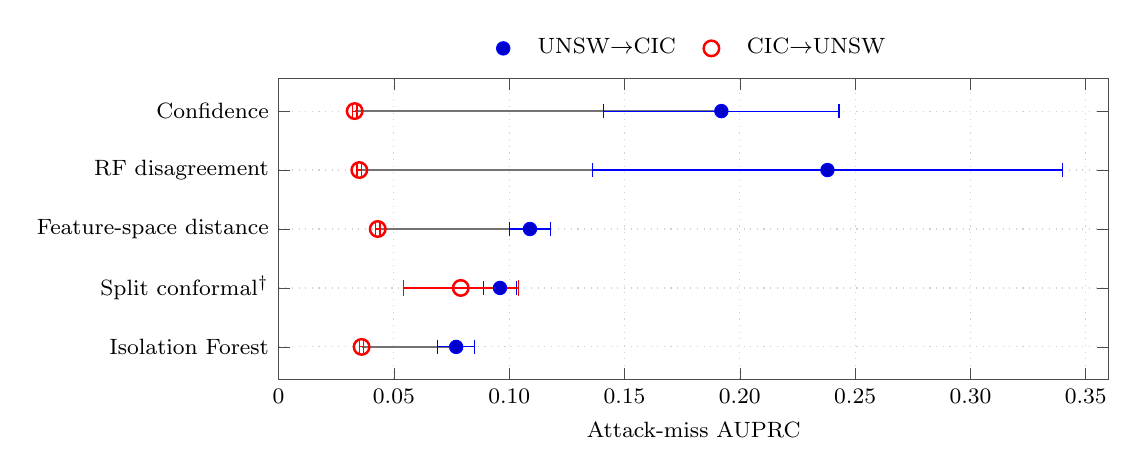
\begin{tikzpicture}
\begin{axis}[
  width=\columnwidth,
  height=5.4cm,
  xmin=0, xmax=0.36,
  ymin=0.45, ymax=5.55,
  xlabel={Attack-miss AUPRC},
  ylabel={},
  xtick={0,0.05,0.10,0.15,0.20,0.25,0.30,0.35},
  xticklabels={0,0.05,0.10,0.15,0.20,0.25,0.30,0.35},
  ytick={1,2,3,4,5},
  yticklabels={
    Isolation Forest,
    Split conformal$^\dagger$,
    Feature-space distance,
    RF disagreement,
    Confidence
  },
  y dir=normal,
  grid=major,
  grid style={dotted, draw=black!18},
  axis line style={draw=black!70},
  tick style={draw=black!70},
  label style={font=\footnotesize},
  tick label style={font=\footnotesize},
  clip=true,
  legend style={
    font=\footnotesize,
    at={(0.5,1.03)},
    anchor=south,
    legend columns=2,
    draw=none,
    column sep=0.8em
  },
  clip=false
]

% Directional connecting segments.
\addplot[black!55, line width=0.8pt, forget plot]
  coordinates {(0.077,1) (0.036,1)};
\addplot[black!55, line width=0.8pt, forget plot]
  coordinates {(0.096,2) (0.079,2)};
\addplot[black!55, line width=0.8pt, forget plot]
  coordinates {(0.109,3) (0.043,3)};
\addplot[black!55, line width=0.8pt, forget plot]
  coordinates {(0.238,4) (0.035,4)};
\addplot[black!55, line width=0.8pt, forget plot]
  coordinates {(0.192,5) (0.033,5)};

% UNSW -> CIC: filled markers with SD error bars.
\addplot+[
  only marks,
  mark=*,
  mark size=2.4pt,
  error bars/.cd,
  x dir=both,
  x explicit
] coordinates {
  (0.077,1) +- (0.008,0)
  (0.096,2) +- (0.007,0)
  (0.109,3) +- (0.009,0)
  (0.238,4) +- (0.102,0)
  (0.192,5) +- (0.051,0)
};
\addlegendentry{UNSW$\rightarrow$CIC}

% CIC -> UNSW: open markers with SD error bars.
\addplot+[
  only marks,
  mark=o,
  mark size=2.8pt,
  mark options={line width=0.9pt},
  error bars/.cd,
  x dir=both,
  x explicit
] coordinates {
  (0.036,1) +- (0.001,0)
  (0.079,2) +- (0.025,0)
  (0.043,3) +- (0.001,0)
  (0.035,4) +- (0.001,0)
  (0.033,5) +- (0.001,0)
};
\addlegendentry{CIC$\rightarrow$UNSW}

\end{axis}
\end{tikzpicture}%
}
\caption{Bidirectional attack-miss AUPRC. Filled and open markers denote the two transfer directions; horizontal error bars show seed-level standard deviation. Each segment connects the two directional means for the same reliability signal, making directional transportability visible without replacing the exact values reported in Table~IV.}
\label{fig:bidirectional-auprc}
\end{figure}

In UNSW$\rightarrow$CIC, RF disagreement achieves the highest mean attack-miss AUPRC at 0.238. In CIC$\rightarrow$UNSW, the ordering changes and feature-space distance is the highest non-conformal signal at 0.043. The split-conformal value of 0.079 is retained for audit completeness but is not interpreted as a competitive result because its scalar is degenerate. Thus, the best-performing reliability mechanism is not invariant to reversal of the source and target domains.

The figure also makes the different directional behavior of the non-degenerate signals apparent. RF disagreement and confidence move substantially between the two directions, whereas feature-space distance changes less in threshold-free ranking. The conformal points are shown only as an audit reference. Feature-space distance and Isolation Forest remain lower-performing signals in both directions despite their different directional changes.

The paired seed analysis provides inferential support for the strongest UNSW$\rightarrow$CIC contrasts. RF disagreement exceeds confidence by a mean paired difference of 0.046, with a 95\% bootstrap interval excluding zero. The earlier RF-versus-conformal contrast is not used as a primary superiority claim because the conformal scalarization is tie-dominated. These effects are reported alongside the broader multiple-comparison analysis rather than interpreted as evidence of a universal ranking.

The primary endpoint establishes the first central result of the study: reliability performance is source-target-direction dependent, but its interpretation must be conditioned on detector transfer failure and on the validity of each reliability score's scalarization. A ranking obtained from one transfer direction cannot automatically be treated as a transportable ordering for the reverse deployment direction.

\subsection{Operational Utility at Fixed Analyst-Review Budgets}

The primary operational analysis asks how many detector attack misses can be recovered when only a fixed fraction of the complete target-flow population can be reviewed. The benchmark is deliberately a whole-target ranking abstraction rather than a predicted-benign SOC queue. Fig.~2 plots the budget-response curves for the two transfer directions, making changes in operational ranking visible across review capacity. Table~V reports the exact mean capture values at the 1\%, 5\%, and 10\% budgets.

\begin{figure*}[!t]
\centering
\resizebox{0.92\textwidth}{!}{%
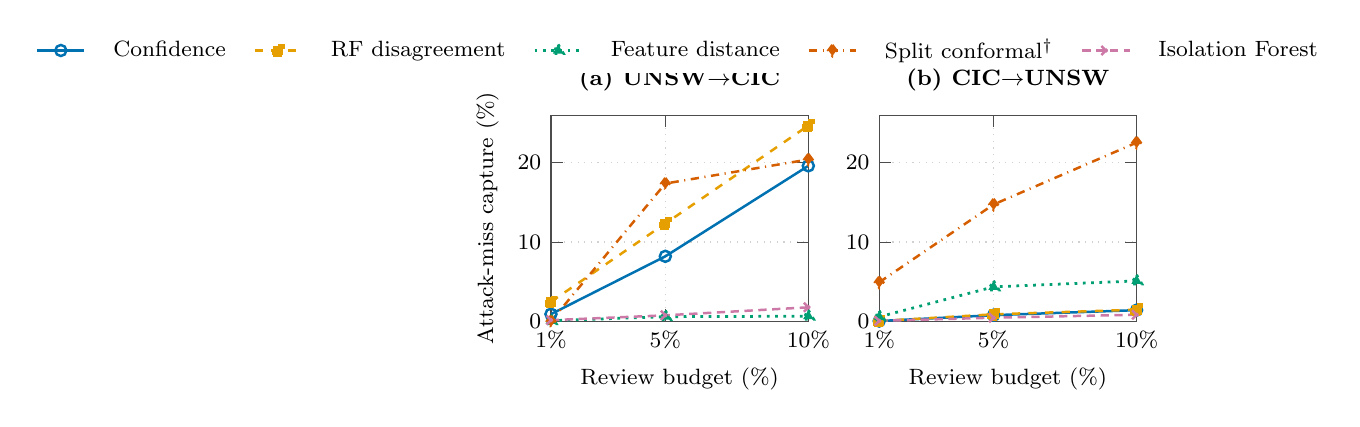
\begin{tikzpicture}
\begin{groupplot}[
  group style={
    group size=2 by 1,
    horizontal sep=0.9cm
  },
  width=0.40\textwidth,
  height=4.2cm,
  xmin=1, xmax=10,
  ymin=0, ymax=26,
  xtick={1,5,10},
  xticklabels={1\%,5\%,10\%},
  xlabel={Review budget (\%)},
  ylabel={Attack-miss capture (\%)},
  grid=major,
  grid style={dotted, draw=black!18},
  axis line style={draw=black!70},
  tick style={draw=black!70},
  label style={font=\footnotesize},
  tick label style={font=\footnotesize},
  legend style={
    font=\footnotesize,
    at={(0.5,1.20)},
    anchor=south,
    legend columns=5,
    draw=none,
    column sep=0.8em
  },
  clip=true
]

\nextgroupplot[
  title={(a) UNSW$\rightarrow$CIC},
  title style={font=\footnotesize\bfseries, yshift=-1pt}
]

% Confidence
\addplot[solid,mark=o,mark size=2pt,line width=0.9pt,color=methodblue]
  coordinates {(1,0.90) (5,8.19) (10,19.60)};
\addlegendentry{Confidence}

% RF disagreement
\addplot[dashed,mark=square*,mark size=1.8pt,line width=0.9pt,color=methodorange]
  coordinates {(1,2.46) (5,12.33) (10,24.68)};
\addlegendentry{RF disagreement}

% Feature distance
\addplot[dotted,mark=triangle*,mark size=2.2pt,line width=1.0pt,color=methodgreen]
  coordinates {(1,0.07) (5,0.58) (10,0.64)};
\addlegendentry{Feature distance}

% Split conformal
\addplot[dashdotted,mark=diamond*,mark size=2.0pt,line width=0.9pt,color=methodvermillion]
  coordinates {(1,0.0001) (5,17.37) (10,20.40)};
\addlegendentry{Split conformal$^\dagger$}

% Isolation Forest
\addplot[densely dashed,mark=x,mark size=2.3pt,line width=0.9pt,color=methodpurple]
  coordinates {(1,0.14) (5,0.75) (10,1.76)};
\addlegendentry{Isolation Forest}

\nextgroupplot[
  title={(b) CIC$\rightarrow$UNSW},
  title style={font=\footnotesize\bfseries, yshift=-1pt},
  ylabel={}
]

% Same styles, no repeated legend.
\addplot[solid,mark=o,mark size=2pt,line width=0.9pt,color=methodblue,forget plot]
  coordinates {(1,0.03) (5,0.77) (10,1.40)};
\addplot[dashed,mark=square*,mark size=1.8pt,line width=0.9pt,color=methodorange,forget plot]
  coordinates {(1,0.03) (5,0.88) (10,1.46)};
\addplot[dotted,mark=triangle*,mark size=2.2pt,line width=1.0pt,color=methodgreen,forget plot]
  coordinates {(1,0.56) (5,4.34) (10,5.09)};
\addplot[dashdotted,mark=diamond*,mark size=2.0pt,line width=0.9pt,color=methodvermillion,forget plot]
  coordinates {(1,4.91) (5,14.73) (10,22.53)};
\addplot[densely dashed,mark=x,mark size=2.3pt,line width=0.9pt,color=methodpurple,forget plot]
  coordinates {(1,0.05) (5,0.45) (10,0.82)};

\end{groupplot}
\end{tikzpicture}
}
\caption{Attack-miss capture as a function of analyst-review budget. Each panel corresponds to one transfer direction; line style and marker identify the reliability signal, with color providing redundant visual separation. The curves show that operational ranking changes with review capacity and need not match the threshold-free attack-miss AUPRC ordering.}
\label{fig:budget-capture}
\end{figure*}

\begin{table*}[!t]
\centering
\caption{Attack-miss capture at fixed review budgets}
\begin{adjustbox}{max width=\textwidth}
\begin{tabular}{lllllll}
\toprule
\textbf{Reliability signal} & \textbf{UNSW->CIC 1\%} & \textbf{UNSW->CIC 5\%} & \textbf{UNSW->CIC 10\%} & \textbf{CIC->UNSW 1\%} & \textbf{CIC->UNSW 5\%} & \textbf{CIC->UNSW 10\%} \\
\midrule
Confidence & 0.90\% & 8.19\% & 19.60\% & 0.03\% & 0.77\% & 1.40\% \\
RF disagreement & 2.46\% & 12.33\% & 24.68\% & 0.03\% & 0.88\% & 1.46\% \\
Feature-space distance & 0.07\% & 0.58\% & 0.64\% & 0.56\% & 4.34\% & 5.09\% \\
Split conformal$^\dagger$ & 0.0001\% & \textbf{17.37\%} & 20.40\% & \textbf{4.91\%} & \textbf{14.73\%} & \textbf{22.53\%} \\
Isolation Forest & 0.14\% & 0.75\% & 1.76\% & 0.05\% & 0.45\% & 0.82\% \\
\bottomrule
\end{tabular}
\end{adjustbox}
\end{table*}



At the primary 5\% review budget, the random-review baseline is 5\% capture. Among the non-degenerate signals, RF disagreement captures 12.33\% in UNSW$\rightarrow$CIC, while feature-space distance captures 4.34\% in CIC$\rightarrow$UNSW and is therefore below the random baseline. The split-conformal 17.37\% and 14.73\% values are retained for audit completeness but are not interpreted as comparative evidence because the score is dominated by equal-value ties. In the first direction, this differs from the AUPRC result in Fig.~1, where RF disagreement has the highest threshold-free ranking performance. The two metrics therefore identify different aspects of operational usefulness.

Fig.~2 further shows that operational ordering changes with review capacity. A 5\% budget corresponds to approximately 1,005,776 CIC target flows and 118,271 UNSW target flows. In UNSW$\rightarrow$CIC, RF disagreement and confidence are the strongest non-degenerate operational signals, while distance and Isolation Forest are near or below random review. In CIC$\rightarrow$UNSW, distance is the strongest non-conformal signal and modestly exceeds the random baseline at 5\% review.

The paired analysis is restricted to predeclared non-degenerate contrasts. Conformal contrasts are not treated as substantive method comparisons because of the scalarization audit. The deterministic tie rule is also a limitation for RF disagreement and conformal, so randomized-tie sensitivity is required.

At 5\% review, mean residual attack-miss rate among unreviewed flows was approximately 8.9\% for RF disagreement, 9.3\% for confidence, 10.1\% for distance, and 10.0\% for Isolation Forest in UNSW$\rightarrow$CIC; in CIC$\rightarrow$UNSW the corresponding values were about 5.6\%, 5.6\%, 5.4\%, and 5.7\%. These selective-risk quantities are secondary because the review pool is the complete target population. Threshold-free ranking and fixed-budget triage should consequently be reported as complementary, rather than interchangeable, evaluations.

\subsection{Generic Errors Versus Security-Critical Attack Misses}

The generic-error analysis asks whether a reliability signal that is effective at identifying incorrect detector predictions is necessarily effective at prioritizing the subset of those errors that are attacks classified as benign. Generic-error prevalence is approximately 51.8\% in UNSW$\rightarrow$CIC and 5.40\% in CIC$\rightarrow$UNSW. Fig.~3 visualizes the relationship between generic-error and attack-miss AUPRC directly. Table~VI reports the corresponding exact AUPRC and AUROC values.

\begin{figure*}[t]
\centering
\resizebox{0.92\textwidth}{!}{%
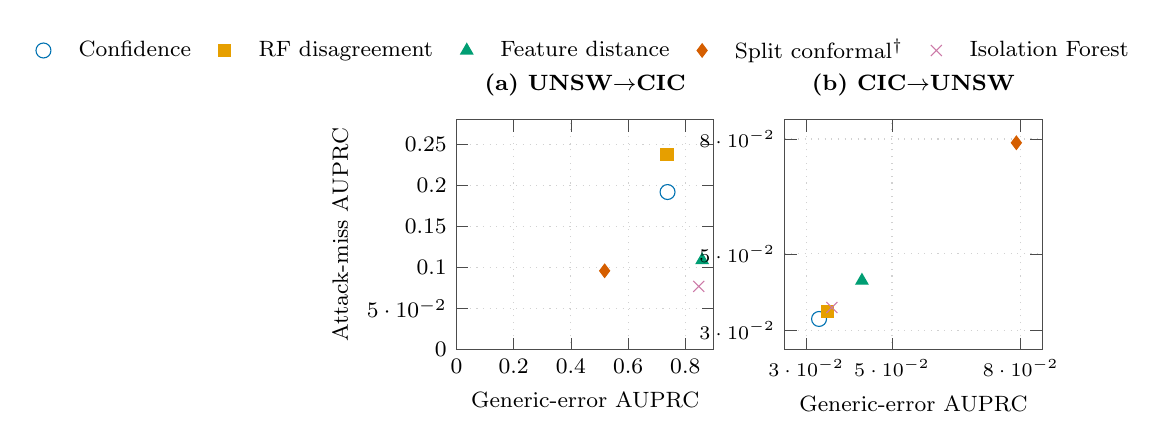
\begin{tikzpicture}
\begin{groupplot}[
  group style={
    group size=2 by 1,
    horizontal sep=0.9cm
  },
  width=0.40\textwidth,
  height=4.5cm,
  xmin=0, xmax=0.90,
  ymin=0, ymax=0.28,
  xtick={0,0.2,0.4,0.6,0.8},
  ytick={0,0.05,0.10,0.15,0.20,0.25},
  xlabel={Generic-error AUPRC},
  ylabel={Attack-miss AUPRC},
  grid=major,
  grid style={dotted, draw=black!18},
  axis line style={draw=black!70},
  tick style={draw=black!70},
  label style={font=\footnotesize},
  tick label style={font=\footnotesize},
  scaled y ticks=false,
  clip=true,
]

\nextgroupplot[
  title={(a) UNSW$\rightarrow$CIC},
  title style={font=\footnotesize\bfseries, yshift=-1pt},
  legend style={
    font=\footnotesize,
    at={(0.5,1.20)},
    anchor=south,
    legend columns=5,
    draw=none,
    column sep=0.8em
  }
]

\addplot[only marks,mark=o,mark size=2.7pt,color=methodblue]
  coordinates {(0.738,0.192)};
\addlegendentry{Confidence}

\addplot[only marks,mark=square*,mark size=2.2pt,color=methodorange]
  coordinates {(0.736,0.238)};
\addlegendentry{RF disagreement}

\addplot[only marks,mark=triangle*,mark size=2.5pt,color=methodgreen]
  coordinates {(0.859,0.109)};
\addlegendentry{Feature distance}

\addplot[only marks,mark=diamond*,mark size=2.4pt,color=methodvermillion]
  coordinates {(0.518,0.096)};
\addlegendentry{Split conformal$^\dagger$}

\addplot[only marks,mark=x,mark size=2.8pt,color=methodpurple]
  coordinates {(0.847,0.077)};
\addlegendentry{Isolation Forest}

\nextgroupplot[
  title={(b) CIC$\rightarrow$UNSW},
  title style={font=\footnotesize\bfseries, yshift=-1pt},
  ylabel={},
  xmin=0.025, xmax=0.085,
  ymin=0.025, ymax=0.085,
  xtick={0.03,0.05,0.08},
  ytick={0.03,0.05,0.08},
  tick label style={font=\scriptsize},
  scaled x ticks=false,
  scaled y ticks=false
]

\addplot[only marks,mark=o,mark size=2.7pt,color=methodblue,forget plot]
  coordinates {(0.033,0.033)};
\addplot[only marks,mark=square*,mark size=2.2pt,color=methodorange,forget plot]
  coordinates {(0.035,0.035)};
\addplot[only marks,mark=triangle*,mark size=2.5pt,color=methodgreen,forget plot]
  coordinates {(0.043,0.043)};
\addplot[only marks,mark=diamond*,mark size=2.4pt,color=methodvermillion,forget plot]
  coordinates {(0.079,0.079)};
\addplot[only marks,mark=x,mark size=2.8pt,color=methodpurple,forget plot]
  coordinates {(0.036,0.036)};

\end{groupplot}
\end{tikzpicture}%
}
\caption{Relationship between generic-error and attack-miss AUPRC. Each point represents one reliability signal; marker shape identifies the signal, with color providing redundant visual separation. The right panel uses a narrower axis range to resolve the closely clustered CIC$\rightarrow$UNSW values; its plotted values remain the same as in Table~VI. The UNSW$\rightarrow$CIC panel shows that strong generic-error ranking need not imply strong attack-miss ranking, while the CIC$\rightarrow$UNSW panel shows the two metrics becoming nearly identical for all five signals.}
\label{fig:generic-vs-attackmiss}
\end{figure*}

\begin{table*}[!t]
\centering
\caption{Generic error and attack-miss behavior}
\begin{adjustbox}{max width=\textwidth}
\begin{tabular}{lllllll}
\toprule
\textbf{Signal} & \textbf{UNSW->CIC generic-error AUPRC} & \textbf{UNSW->CIC attack-miss AUPRC} & \textbf{UNSW->CIC attack-miss AUROC} & \textbf{CIC->UNSW generic-error AUPRC} & \textbf{CIC->UNSW attack-miss AUPRC} & \textbf{CIC->UNSW attack-miss AUROC} \\
\midrule
Confidence & 0.738 & 0.192 & 0.701 & 0.033 & 0.033 & 0.228 \\
RF disagreement & 0.736 & 0.238 & 0.712 & 0.035 & 0.035 & 0.248 \\
Feature-space distance & 0.859 & 0.109 & 0.575 & 0.043 & 0.043 & 0.345 \\
Split conformal$^\dagger$ & 0.518 & 0.096 & 0.500 & 0.079 & 0.079 & \textbf{0.545} \\
Isolation Forest & 0.847 & 0.077 & 0.379 & 0.036 & 0.036 & 0.284 \\
\bottomrule
\end{tabular}
\end{adjustbox}
\end{table*}



The UNSW$\rightarrow$CIC direction provides the clearest separation between generic error detection and security-specific attack-miss prioritization. Fig.~3 shows that feature-space distance and Isolation Forest lie at the high end of generic-error AUPRC while remaining substantially lower on attack-miss AUPRC. Their generic-error AUPRC values are 0.859 and 0.847, but their attack-miss AUPRC values fall to 0.109 and 0.077. By contrast, RF disagreement and confidence achieve somewhat lower generic-error AUPRC but substantially higher attack-miss AUPRC.

This divergence means that input atypicality and security-critical detector failure are not interchangeable reliability objectives. An observation can be unusual in the selected feature space without being an attack that the detector misses, while an attack miss can remain close to source traffic and receive only a modest novelty score.

Split conformal's generic-error AUPRC in UNSW$\rightarrow$CIC is 0.518, essentially its generic-error prevalence, while its generic-error and attack-miss AUROCs are both approximately 0.500. This is consistent with the scalarization audit rather than evidence of a meaningful reliability ranking.

The reverse CIC$\rightarrow$UNSW direction has a different structure. The detector is effectively blind to attacks, so generic errors and attack misses almost coincide. Generic-error and attack-miss AUROC are approximately 0.228/0.228 for confidence, 0.248/0.248 for RF disagreement, 0.345/0.345 for distance, and 0.284/0.284 for Isolation Forest. In this target setting, generic errors are therefore largely accounted for by attack misses, making the generic-error metric a poor independent test of security-specific reliability.

The UNSW$\rightarrow$CIC results show that generic-error discrimination can survive while security-specific ranking deteriorates: generic-error AUROC averages about 0.839, 0.837, 0.877, and 0.840 for confidence, RF disagreement, distance, and Isolation Forest, while attack-miss AUROC falls to about 0.701, 0.712, 0.575, and 0.379. In CIC$\rightarrow$UNSW, four non-conformal signals are below 0.5, but this inversion is inseparable from the near-blind detector regime.

The results therefore show that generic prediction-error ranking is insufficient as a security-reliability validation target, consistent with the broader distinction between detecting misclassified examples and detecting the particular failure mode that matters operationally [22]. A signal can perform strongly on ordinary detector errors while performing poorly on dangerous attack misses. The primary reliability question should consequently be defined by the security failure mode that the analyst workflow is intended to recover.

\subsection{Directional Transportability of Reliability Performance}

Fig.~1 shows the directional change in attack-miss AUPRC directly; Table~VII expresses the primary metrics relative to direction-specific baselines because attack-miss prevalence differs materially between the two targets.

\begin{table}[t]
\centering
\caption{Direction-normalized reliability performance}
\begin{adjustbox}{max width=\columnwidth}
\begin{tabular}{lll}
\toprule
\textbf{Signal} & \textbf{AUPRC lift (UNSW/CIC)} & \textbf{5\% capture lift (UNSW/CIC)} \\
\midrule
Confidence & 2.00 / 0.61 & 1.64 / 0.15 \\
RF disagreement & \textbf{2.47 / 0.64} & \textbf{2.47 / 0.18} \\
Feature-space distance & 1.13 / 0.80 & 0.12 / 0.87 \\
Split conformal$^\dagger$ & 1.00 / 1.47 & 3.47 / 2.95 \\
Isolation Forest & 0.80 / 0.66 & 0.15 / 0.09 \\
\bottomrule
\end{tabular}
\end{adjustbox}
\\[-1mm]
{\footnotesize AUPRC lift is relative to attack-miss prevalence; 5\% capture lift is relative to random 5\% review. Pairs are UNSW$\rightarrow$CIC / CIC$\rightarrow$UNSW. $^\dagger$ Conformal is audit-only.}
\end{table}

RF disagreement retains the strongest normalized threshold-free lift in UNSW$\rightarrow$CIC, while distance becomes relatively stronger for the fixed-budget endpoint in CIC$\rightarrow$UNSW. The normalized view is preferable to raw directional gaps because the positive-event prevalence differs by direction.

Conformal's normalized values are shown for audit completeness only. Isolation Forest has low absolute and normalized operational utility in both directions, so its small raw directional gap does not imply useful transportability.

The directional results therefore distinguish \textbf{absolute utility} from \textbf{transport stability}. A signal may achieve strong performance in one direction but change substantially after source-target reversal, or it may remain relatively stable while providing limited security value. This is why a one-way transfer experiment cannot establish that a reliability ranking is transportable.

\subsection{Family-Level Analysis and Scope of Interpretation}

Family-level analysis is restricted to the frozen cross-domain semantic registry. Only the documented shared DoS category is treated as a defensible cross-dataset correspondence; dataset-local attack names are not treated as equivalent merely because their labels are similar.

The available family evidence is insufficient for a broad family-level conclusion. The locked semantic registry admits only the documented shared DoS relation; other target families are not called unseen because unsupported semantic mappings are intentionally withheld. In UNSW$\rightarrow$CIC, the shared DoS mapping contains no target rows. In CIC$\rightarrow$UNSW, all 5,980 mapped DoS target rows are recorded as attack misses, producing an attack-miss AUPRC of 1.0 for every reliability signal. Because every mapped row belongs to the positive attack-miss population, this value is tautological rather than evidence of method superiority.

Accordingly, the family analysis is not used to support claims about general unseen-family detection or family-specific reliability robustness. Its role is instead to establish an interpretive boundary: meaningful cross-domain family analysis requires both a defensible semantic correspondence and sufficient within-family variation in detector outcomes.

The experiment therefore provides evidence about source-only cross-domain reliability transportability at the aggregate security-failure level, but it does not establish comprehensive unseen-family generalization.

\subsection{Calibration and Conformal Diagnostics}

Calibration behavior differs between the two transfer directions. For UNSW$\rightarrow$CIC, the mean target Brier score across the ten seeds is 0.245 and the mean 15-bin expected calibration error (ECE) is 0.317. For CIC$\rightarrow$UNSW, the corresponding descriptive values are 0.075 and 0.153. These quantities are reported as secondary diagnostics because calibration quality is distinct from the primary task of prioritizing detector attack misses.

The calibration results provide context for the confidence signal but do not alter the primary ranking analysis. In particular, the study does not assume that source-calibrated probability values retain their numerical target-domain interpretation after transfer.

 The conformal diagnostic requires a stronger correction than the earlier draft implied.
 The archived target set-size output is not merely a malformed ambiguity statistic: the prediction sets are overwhelmingly empty or singleton, so the saved scalar (r=|C|-1) collapses to (-1) or (0). The resulting cutoff tie mass is enormous; at 5\% review, essentially the full target population can share the conformal cutoff score. The archived capture values therefore depend on deterministic row-offset tie handling.

 Accordingly, conformal AUPRC and capture are retained only as audit outputs. They are not used to establish method superiority or transport stability. A corrected experiment should replace the binary set-size scalar with a continuous conformal p-value or nonconformity ranking and report randomized-tie or expected-tie budget capture before comparative conclusions are drawn.

 The distinction is important because classical conformal guarantees depend on conditions such as exchangeability [26]. The present cross-domain experiment does not establish that those conditions hold on the target domain. The paper therefore reports empirical ranking and triage behavior without interpreting it as a target-domain conformal guarantee.

\subsection{Paired Effects Across Random Seeds}

The ten-seed design permits matched comparisons because the same detector seed is used for every reliability method within a transfer direction. Table~VIII reports selected paired contrasts using the mean seed-level difference, a seed-level bootstrap interval, and an exact two-sided sign-flip permutation test.

\begin{table}[t]
\centering
\caption{Selected paired effects}
\begin{adjustbox}{max width=\columnwidth}
\begin{tabular}{llllll}
\toprule
\textbf{Direction} & \textbf{Comparison} & \textbf{Metric} & \textbf{Mean difference} & \textbf{Bootstrap interval} & \textbf{Exact p} \\
\midrule
UNSW->CIC & RF disagreement - split conformal & Attack-miss AUPRC & +0.142 & [0.082, 0.206] & 0.00195 \\
UNSW->CIC & RF disagreement - split conformal & 5\% capture & -0.050 & [-0.110, 0.016] & 0.168 \\
CIC->UNSW & RF disagreement - split conformal & Attack-miss AUPRC & -0.045 & [-0.061, -0.031] & 0.00195 \\
CIC->UNSW & Feature distance - split conformal & Attack-miss AUPRC & -0.036 & [-0.052, -0.023] & 0.00195 \\
CIC->UNSW & RF disagreement - split conformal & 5\% capture & -0.139 & [-0.169, -0.111] & 0.00195 \\
UNSW->CIC & RF disagreement - confidence & Attack-miss AUPRC & +0.046 & [0.014, 0.088] & 0.00781 \\
\bottomrule
\end{tabular}
\end{adjustbox}
\end{table}

The paired effects reinforce the contrast already visible in Figs.~1 and~2. In UNSW$\rightarrow$CIC, RF disagreement has a mean paired AUPRC advantage over confidence of 0.046 with a bootstrap interval excluding zero. The earlier RF-versus-conformal contrast is retained only as an audit statistic because the conformal score is tie-dominated.

In CIC$\rightarrow$UNSW, feature-space distance is the strongest non-conformal attack-miss AUPRC signal, while conformal paired contrasts are not used to support a preferred-method claim.

These tests support selected method contrasts but do not establish a single global ordering across all signals and metrics. The broader pairwise results are retained in the analysis artifacts, while the manuscript emphasizes effect magnitudes, uncertainty intervals, directional consistency, and the operational patterns shown in Figs.~1--3.

\subsection{Computational Cost}

Computational cost is treated as a secondary deployment consideration rather than a scientific factor. The execution-level Random Forest parallelism benchmark compared multiple worker settings against a single-worker reference and verified exact equivalence of tree structure, class probabilities, and RF disagreement.

In the bounded CIC benchmark, RF fitting time decreased from 17.64~s at 10 workers to 16.50~s at 16 workers, while CPU saturation increased substantially. The production setting therefore used 10 workers, which provided most of the available parallel speedup without the near-total CPU saturation observed at the highest tested settings.

This benchmark separates execution efficiency from the scientific definition of the detector. Worker parallelism changes runtime but, under the verified equivalence condition, does not change the model being evaluated. No figure is used because the benchmark is not central to the scientific conclusions and the two timing values are more precisely reported in text.

\section{Discussion}

\subsection{Principal Findings}

It does not identify a universally transportable reliability signal. The completed bidirectional experiment instead reveals three interacting patterns: the detector itself can collapse under transfer, non-degenerate reliability signals can change ranking with direction, and generic-error ranking can diverge from security-specific attack-miss prioritization. Fig.~1 shows that the relative attack-miss AUPRC ranking changes when the source and target domains are reversed. Fig.~2 shows that operational capture also depends on the review budget and random-review baseline. Fig.~3 shows that generic prediction-error ranking can diverge substantially from security-specific attack-miss ranking.

Together, these findings support the central interpretation that reliability transportability is not a property of a score in isolation. It depends on the interaction among the detector, source and target distributions, reliability construction, security failure mode, and operational review budget. A reliability layer selected from one benchmark direction therefore cannot automatically be treated as deployment-robust.

\subsection{Why Generic Reliability and Security Reliability Diverge}

Fig.~3 provides the clearest evidence for the distinction between generic reliability and security-specific reliability. In UNSW$\rightarrow$CIC, feature-space distance and Isolation Forest occupy relatively strong positions on generic-error AUPRC while remaining much lower on attack-miss AUPRC. This pattern is consistent with a difference between \textbf{input atypicality} and \textbf{security-relevant detector failure}.

An observation can be unusual in the chosen feature space without being an attack that the detector misses. Conversely, a dangerous attack can remain close to source traffic and therefore receive a modest novelty score. The figure therefore supports a narrower interpretation of novelty signals: they measure atypicality under the selected representation, not security risk itself.

The behavior of RF disagreement is consistent with a different mechanism. It is generated directly from the detector ensemble and reflects instability of the classifier's decision process rather than only the atypicality of the input representation. Its comparatively favorable attack-miss position in UNSW$\rightarrow$CIC is therefore consistent with model-dependent uncertainty sometimes being more aligned with detector failure than representation-level novelty. This remains an empirical association rather than a demonstrated causal mechanism.

The reverse direction adds a separate semantic concern. The attack-miss AUROC results show that several scores become systematically anti-informative when the same high-score review convention is transferred from CIC$\rightarrow$UNSW. Thus, a reliability score can fail not only by becoming weak but by changing the direction in which it should be interpreted.

\subsection{Interpreting the Conformal Result}

The conformal arm should be interpreted as an implementation audit rather than as a validated competitive reliability result. The source calibration is correctly source-only, but the exported prediction-set-size scalar collapses to a highly tied \(-1/0\) variable. This explains the near-zero target set sizes and abrupt budget-capture behavior. The result demonstrates that a conformal method cannot be judged from its nominal coverage parameter alone; the exported ranking scalar must be non-degenerate under the deployment setting.

Classical conformal guarantees depend on exchangeability, and the present transfer setting does not establish target exchangeability [27]. A corrected continuous-score conformal rerun is required before the method can be compared fairly with the other signals.

\subsection{Implications for Deployment}

The results suggest that deployment monitoring should answer two separate questions before a reliability score is used to prioritize analyst attention.

First, \textbf{does the score remain aligned with actual detector failures after transfer?} The directional and semantic behavior in Fig.~1 and the attack-miss AUROC analysis show that this cannot be assumed.

Second, \textbf{how useful is the score under the available analyst budget?} Fig.~2 demonstrates that operational capture depends on the review fraction and need not follow the threshold-free AUPRC ranking.

These observations imply that an offline validation study with trusted deployment labels should verify score orientation and budgeted capture before operationalizing a source-only reliability layer. The source-only runtime protocol itself does not require those labels; they are needed for external validation of the failure-detection objective. The appropriate validation target should be the security failure mode of interest—here, attack misses—rather than generic error detection alone, as demonstrated in Fig.~3.

The present study does not imply that source-only reliability monitoring is a substitute for target-domain adaptation. Instead, it provides a measurement baseline for the case in which adaptation is unavailable, delayed, undesirable, or deliberately excluded. Where target information later becomes available, future work can investigate whether calibration or score orientation can be improved without weakening the source-only leakage controls used here.

\subsection{Relationship to Existing Literature}

The results reinforce several conclusions emerging from recent work while contributing a narrower security-focused evaluation. Recent studies already show that cross-dataset and temporal shift can damage confidence, threshold transfer, and label-free monitoring [1], [2]. Recent conformal IDS work similarly shows that novelty and triage behavior can vary across attack families [7].

The present study extends that picture by evaluating reliability specifically against the detector's \textbf{attack misses}, while holding the detector and source-derived reliability layer fixed and reversing the transfer direction. The contribution is therefore empirical and integrative rather than algorithmic: it demonstrates how transportability, operational budget, and security-specific error definition jointly change the interpretation of existing post-hoc reliability signals.

\subsection{Future Research Directions}

The results point to several high-value extensions.

\textbf{Temporal deployment drift:} The current experiment compares two cross-domain environments. A natural extension is to evaluate the same reliability layers as source calibration becomes stale over time, explicitly separating temporal drift from cross-dataset differences [1].

\textbf{Target-label-efficient recalibration:} The source-only protocol intentionally prevents target recalibration. Future work can quantify how much trusted target information is needed to recover score orientation or calibration without requiring full retraining.

\textbf{Broader domain replication:} Repeating the experiment across additional NetFlow-v3 domains and other common-feature IDS benchmarks would test whether the observed direction dependence is specific to the present pair or represents a broader phenomenon.

\textbf{Family-conditional reliability:} A larger, independently validated attack-family ontology could determine whether reliability transportability differs systematically by attack semantics rather than restricting family analysis to the single defensible shared category available here.

\textbf{Composite reliability policies:} The present study compares individual signals. Future work could test whether combinations of disagreement, calibrated confidence, and feature-space novelty yield more stable triage than individual scores while preserving source-only constraints.

\section{Limitations}

\subsection{Dataset and Domain Scope}

The primary conclusions are based on two NetFlow-v3 datasets and two transfer directions. Although the use of a common feature interface reduces one major source of incompatibility, two benchmark environments cannot establish universal transportability across network types, organizations, traffic-generating applications, or deployment periods. The findings should therefore be interpreted as controlled evidence for the studied source-target pair rather than as a general guarantee for all NIDS deployments.

\subsection{Fixed Detector Architecture}

The experiment fixes the detector to a Random Forest. This is intentional because it isolates the reliability layer, but it limits architectural generalization. Reliability mechanisms may interact differently with neural detectors, gradient-boosted trees, calibrated linear models, or streaming architectures. The results therefore establish transportability behavior for the studied RF backbone rather than for arbitrary IDS models.

\subsection{Source-Split Duplicate Risk}

The archived 60/20/20 source split hashes the canonical 53-feature representation, while only 46 fields enter the predictive matrix. Although the secondary calibration split groups identical 46-feature vectors together, the primary source partitions could place identical predictor vectors in different train, calibration, and test subsets when only excluded identifier or timestamp fields differ. A duplicate-safe 46-feature source split should therefore be regenerated before final publication.

\subsection{Limited Repetition Count}

Each transfer direction uses ten detector seeds. This provides matched repeated observations for paired analysis but should not be confused with ten independent deployments or ten independent datasets. The seed-level statistical analysis captures detector-training variability under the fixed configuration; it does not quantify variability across organizations, collection campaigns, or network infrastructures.

\subsection{Family-Semantic Coverage}

The attack-family ontology intentionally uses a conservative semantic crosswalk. Only a documented shared DoS category is treated as cross-domain equivalent, and the resulting family analysis is not informative enough to support a general unseen-family conclusion. Many dataset-local attack labels are therefore excluded from direct cross-domain family comparisons.

This limitation is preferable to asserting semantic equivalence from similar names. Nevertheless, it means that the present paper cannot answer how each reliability signal behaves across a comprehensive hierarchy of unseen attack families.

\subsection{Conformal Scalarization and Tie Degeneracy}

The source split-conformal construction is source-only, but its exported prediction-set-size scalar collapses to a highly tied binary score under the present alpha and binary setup. This makes the archived conformal ranking and fixed-budget capture unsuitable for a definitive method comparison until a continuous scalarization and tie-robust analysis are rerun.

\subsection{No Target Adaptation or Recalibration}

The study deliberately forbids target-domain adaptation and recalibration. This is necessary to isolate source-only transportability, but it means the results do not show whether a small amount of target information could substantially improve reliability. In a practical deployment, adaptation, recalibration, threshold adjustment, or continual learning may change the observed ranking.

\subsection{Detector Transfer Failure and Review-Pool Abstraction}

The reverse CIC$\rightarrow$UNSW detector misses essentially all target attacks, so semantic inversion results in that direction must be interpreted as behavior under a near-blind detector rather than as a standalone property of reliability scores. In addition, the review benchmark ranks all target flows; it does not model a predicted-benign analyst queue, alert deduplication, or alert prioritization after already-detected attacks are removed.

\subsection{Benchmark-to-Deployment Gap}

The experiments operate on offline benchmark flow records. They do not model the full operational environment of a live SOC, including analyst fatigue, correlated alerts, changing review capacity, multi-stage incidents, alert deduplication, delayed labels, or adversarial manipulation of the monitoring process. Fixed review budgets are therefore an operational abstraction rather than a complete SOC simulation.

\subsection{Label Quality and Flow Dependence}

The positive class is defined by benchmark labels, and prior audits of public NIDS datasets have documented errors in traffic generation, flow construction, feature extraction, and labeling [31], while later work has explicitly studied label-error prevalence in CIC-IDS2017 and CSE-CIC-IDS2018 [32]. Flows are also not guaranteed to be independent because multiple rows can belong to the same session or temporal episode. Seed-level analysis therefore captures detector-training variability, not all dataset-level uncertainty.

\subsection{Statistical and Multiple-Comparison Constraints}

The analysis includes several methods, metrics, directions, and secondary diagnostics. Pairwise p-values are therefore not interpreted as establishing a single global method ordering. The primary conclusions rely more heavily on effect sizes, paired intervals, direction consistency, and operational behavior than on isolated secondary significance tests.

\subsection{Representation Dependence}

Although the 46-feature interface is standardized across the two primary datasets, distance- and novelty-based reliability mechanisms remain inherently dependent on the chosen feature representation. The present study therefore does not claim representation-invariant reliability. Conclusions about feature-space distance or unsupervised novelty should be interpreted within the frozen representation used here.

\subsection{Researcher-Defined Review Score Orientation}

All methods are normalized to the operational convention that larger scores receive greater review priority. This is necessary for a common budgeted evaluation but means that score orientation is part of the study definition. The semantic-inversion analysis demonstrates why this assumption must be validated under transfer rather than presumed.

Overall, these limitations restrict the scope of the paper's conclusions but do not undermine the central controlled comparison. They define the boundary between what the experiment establishes directly and what requires replication, adaptation experiments, additional datasets, or improved family and conformal validation.

\section{Conclusion}

This study evaluated whether source-fitted post-hoc reliability signals remain useful for prioritizing detector attack misses after a fixed NIDS is transferred to a different domain without target-domain adaptation or recalibration. The source-test baselines show that the Random Forest detector is highly effective in-domain, while the target detector can degrade severely: UNSW$\rightarrow$CIC transfer brings attack discrimination close to chance, and CIC$\rightarrow$UNSW produces an almost completely blind attack detector.

The reliability results therefore cannot be interpreted independently of detector failure. Among the non-degenerate signals, RF disagreement provides the strongest attack-miss AUPRC in UNSW$\rightarrow$CIC, while feature-space distance is the strongest non-conformal signal in CIC$\rightarrow$UNSW. Their relative utility also changes with analyst-review budget and direction-specific random-review baselines. Generic-error performance is not sufficient as a security-reliability proxy: signals can rank ordinary detector errors well while remaining weak on dangerous attack misses.

The conformal arm produces a separate methodological finding rather than a validated method win. Its exported prediction-set-size scalar collapses to a highly tied binary score, making the archived target capture curves dependent on deterministic tie handling. The conformal values are therefore retained for transparency but excluded from comparative superiority claims pending a continuous-score rerun.

The study consequently supports a narrower conclusion than the earlier draft: reliability transportability is deployment- and failure-mode-specific, and it must be evaluated together with detector transfer behavior, direction-specific prevalence, random-review baselines, score tie structure, and operational review definition. The current results also identify two pre-publication requirements---a predictor-space duplicate-safe source split and a corrected continuous conformal scalarization---before the quantitative comparison should be treated as final.

The paper does not establish universal post-hoc reliability robustness, comprehensive unseen-family generalization, or a universal best method. It provides controlled evidence about how existing source-only reliability signals behave under the specific cross-domain transfers studied here and defines the methodological conditions required for a defensible final comparison.
\begin{thebibliography}{32}
\bibitem{1}
W. A. Ahmed, M. A. Rahaman, P. Roy, and P. Alam, ``The dashboard says perfect: A systematic audit of label-free model monitoring and test-time adaptation under temporal distribution shift in network intrusion detection,'' \emph{Frontiers in Artificial Intelligence}, vol. 9, Art. no. 1928858, 2026, doi: 10.3389/frai.2026.1928858.
\bibitem{2}
H. Jin and H. Lee, ``Benchmark-Shift-Aware Intrusion Detection for Evolving Network Traffic: Cross-Dataset Generalization, Calibrated Alerting, and Score-Orientation Diagnostics,'' \emph{Electronics}, vol. 15, no. 17, Art. no. 3761, 2026, doi: 10.3390/electronics15173761.
\bibitem{3}
G. Apruzzese, L. Pajola, and M. Conti, ``The cross-evaluation of machine learning-based network intrusion detection systems,'' \emph{IEEE Trans. Network and Service Management}, vol. 19, no. 4, pp. 5152--5169, 2022, doi: 10.1109/TNSM.2022.3157344.
\bibitem{4}
M. Cantone, C. Marrocco, and A. Bria, ``Machine learning in network intrusion detection: A cross-dataset generalization study,'' \emph{IEEE Access}, vol. 12, Art. no. 144489, 2024, doi: 10.1109/ACCESS.2024.3472907.
\bibitem{5}
E. K. Viegas, A. O. Santin, and L. S. Oliveira, ``Toward a reliable anomaly-based intrusion detection in real-world environments,'' \emph{Computer Networks}, vol. 127, pp. 200--216, 2017, doi: 10.1016/j.comnet.2017.08.013.
\bibitem{6}
E. K. Viegas, A. O. Santin, and P. Tedeschi, ``Toward a reliable evaluation of machine learning schemes for network-based intrusion detection,'' \emph{IEEE Internet of Things Magazine}, vol. 6, no. 2, pp. 70--75, 2023, doi: 10.1109/IOTM.001.2300106.
\bibitem{7}
S. V. Arepalli, U. S. G. Irrinki, A. Morampudi, and R. K. Surapani, ``Conformal prediction for network intrusion triage and analysis of unseen attack families,'' \emph{Discover Informatics}, vol. 1, Art. no. 33, 2026, doi: 10.1007/s44564-026-00033-y.
\bibitem{8}
Y. Ovadia, E. Fertig, J. Ren, Z. Nado, D. Sculley, S. Nowozin, J. V. Dillon, B. Lakshminarayanan, and J. Snoek, ``Can you trust your model's uncertainty? Evaluating predictive uncertainty under dataset shift,'' in \emph{Advances in Neural Information Processing Systems}, vol. 32, 2019.
\bibitem{9}
D. Arp, E. Quiring, F. Pendlebury, A. Warnecke, F. Pierazzi, C. Wressnegger, L. Cavallaro, and K. Rieck, ``Dos and don'ts of machine learning in computer security,'' in \emph{Proc. 31st USENIX Security Symposium}, 2022, pp. 3971--3988.
\bibitem{10}
M. Luay, S. Layeghy, S. Hosseininoorbin, M. Sarhan, N. Moustafa, and M. Portmann, ``Temporal Analysis of NetFlow Datasets for Network Intrusion Detection Systems,'' \emph{IEEE Access}, 2026, doi: 10.1109/ACCESS.2026.3688204.
\bibitem{11}
N. Moustafa and J. Slay, ``UNSW-NB15: a comprehensive data set for network intrusion detection systems (UNSW-NB15 network data set),'' in \emph{Proc. 2015 Military Communications and Information Systems Conf. (MilCIS)}, Canberra, Australia, 2015, pp. 1--6, doi: 10.1109/MilCIS.2015.7348942.
\bibitem{12}
I. Sharafaldin, A. Habibi Lashkari, and A. A. Ghorbani, ``Toward generating a new intrusion detection dataset and intrusion traffic characterization,'' in \emph{Proc. 4th Int. Conf. Information Systems Security and Privacy (ICISSP)}, Funchal, Portugal, 2018, pp. 108--116, doi: 10.5220/0006639801080116.
\bibitem{13}
M. Sarhan, S. Layeghy, and M. Portmann, ``Towards a standard feature set for network intrusion detection system datasets,'' \emph{Mobile Networks and Applications}, vol. 27, pp. 357--370, 2022, doi: 10.1007/s11036-021-01843-0.
\bibitem{14}
T. Saito and M. Rehmsmeier, ``The precision-recall plot is more informative than the ROC plot when evaluating binary classifiers on imbalanced datasets,'' \emph{PLoS ONE}, vol. 10, no. 3, Art. no. e0118432, 2015, doi: 10.1371/journal.pone.0118432.
\bibitem{15}
D. Ha Thanh, ``A transfer-aware, deployment-oriented evaluation framework for NetFlow-based intrusion detection systems (TAN-IDS),'' \emph{PLOS ONE}, vol. 21, no. 4, Art. no. e0346801, 2026, doi: 10.1371/journal.pone.0346801.
\bibitem{16}
D. Ha Thanh, ``Budget-aware two-stage NetFlow intrusion detection for high-traffic critical information infrastructure under domain shift,'' \emph{International Journal of Critical Infrastructure Protection}, vol. 54, 2026, doi: 10.1016/j.ijcip.2026.100876.
\bibitem{17}
H. Li and Z. Zhou, ``From Risk Scores to Budget-Constrained Alert Streams: Temporal Evaluation of Flow-Level Network Intrusion Detection,'' \emph{Electronics}, vol. 15, no. 20, Art. no. 4854, 2026, doi: 10.3390/electronics15204854.
\bibitem{18}
D. Alalisalem, A. Almohsen, K. Albudair, and A. Aljughaiman, ``Cross-Dataset Generalization in Intrusion Detection Systems Using Transfer Learning,'' \emph{IEEE Access}, vol. 14, pp. 90334--90353, 2026, doi: 10.1109/ACCESS.2026.3700037.
\bibitem{19}
C. Guo, G. Pleiss, Y. Sun, and K. Q. Weinberger, ``On calibration of modern neural networks,'' in \emph{Proc. 34th Int. Conf. Machine Learning (ICML)}, PMLR, vol. 70, 2017, pp. 1321--1330.
\bibitem{20}
J. C. Platt, ``Probabilistic outputs for support vector machines and comparisons to regularized likelihood methods,'' in \emph{Advances in Large Margin Classifiers}, MIT Press, 1999, pp. 1--11.
\bibitem{21}
A. Niculescu-Mizil and R. Caruana, ``Predicting good probabilities with supervised learning,'' in \emph{Proc. 22nd Int. Conf. Machine Learning (ICML)}, 2005, pp. 625--632, doi: 10.1145/1102351.1102430.
\bibitem{22}
D. Hendrycks and K. Gimpel, ``A baseline for detecting misclassified and out-of-distribution examples in neural networks,'' in \emph{Proc. Int. Conf. Learning Representations (ICLR)}, 2017.
\bibitem{23}
J. Talpini, F. Sartori, and M. Savi, ``Enhancing trustworthiness in ML-based network intrusion detection with uncertainty quantification,'' \emph{Journal of Reliable Intelligent Environments}, vol. 10, pp. 501--520, 2024, doi: 10.1007/s40860-024-00238-8.
\bibitem{24}
C. K. Chow, ``On optimum recognition error and reject tradeoff,'' \emph{IEEE Trans. Inf. Theory}, vol. 16, no. 1, pp. 41--46, 1970, doi: 10.1109/TIT.1970.1054406.
\bibitem{25}
Y. Geifman and R. El-Yaniv, ``Selective classification for deep neural networks,'' in \emph{Advances in Neural Information Processing Systems 30 (NeurIPS)}, 2017, pp. 4878--4887.
\bibitem{26}
A. N. Angelopoulos and S. Bates, ``A gentle introduction to conformal prediction and distribution-free uncertainty quantification,'' arXiv:2107.07511, 2021.
\bibitem{27}
R. J. Tibshirani, R. Foygel Barber, E. Cand\`es, and A. Ramdas, ``Conformal prediction under covariate shift,'' in \emph{Advances in Neural Information Processing Systems}, vol. 32, pp. 2530--2540, 2019.
\bibitem{28}
F. T. Liu, K. M. Ting, and Z.-H. Zhou, ``Isolation forest,'' in \emph{Proc. 8th IEEE Int. Conf. Data Mining (ICDM)}, 2008, pp. 413--422, doi: 10.1109/ICDM.2008.17.
\bibitem{29}
L. Breiman, ``Random forests,'' \emph{Machine Learning}, vol. 45, no. 1, pp. 5--32, 2001, doi: 10.1023/A:1010933404324.
\bibitem{30}
S. Gautam et al., ``IntrusionDetection: Transportability of Post-Hoc Reliability Signals for Network Intrusion Detection,'' GitHub repository, 2026. [Online]. Available: https://github.com/ShreyasGautam01/IntrusionDetection.
\bibitem{31}
G. Engelen, V. Rimmer, and W. Joosen, ``Troubleshooting an intrusion detection dataset: The CICIDS2017 case study,'' in \emph{Proc. 2021 IEEE Security and Privacy Workshops (SPW)}, 2021, pp. 7--12, doi: 10.1109/SPW53761.2021.00009.
\bibitem{32}
L. Liu, G. Engelen, T. Lynar, D. Essam, and W. Joosen, ``Error prevalence in NIDS datasets: A case study on CIC-IDS-2017 and CSE-CIC-IDS-2018,'' in \emph{Proc. 2022 IEEE Conf. Communications and Network Security (CNS)}, 2022, pp. 254--263, doi: 10.1109/CNS56114.2022.9947235.
\end{thebibliography}
\end{document}